\documentclass[tikz,border=2pt]{standalone}
\usepackage{amsmath,amssymb}
\usepackage{tikz}
\usetikzlibrary{arrows.meta}

\begin{document}
% A diet problem: minimise feed cost 2 x_A + 3 x_B subject to calorie and vitamin
% requirements (>= constraints). The feasible region is unbounded above; the cheapest point is
% the corner (1.2, 2.4) where both requirements are met exactly.
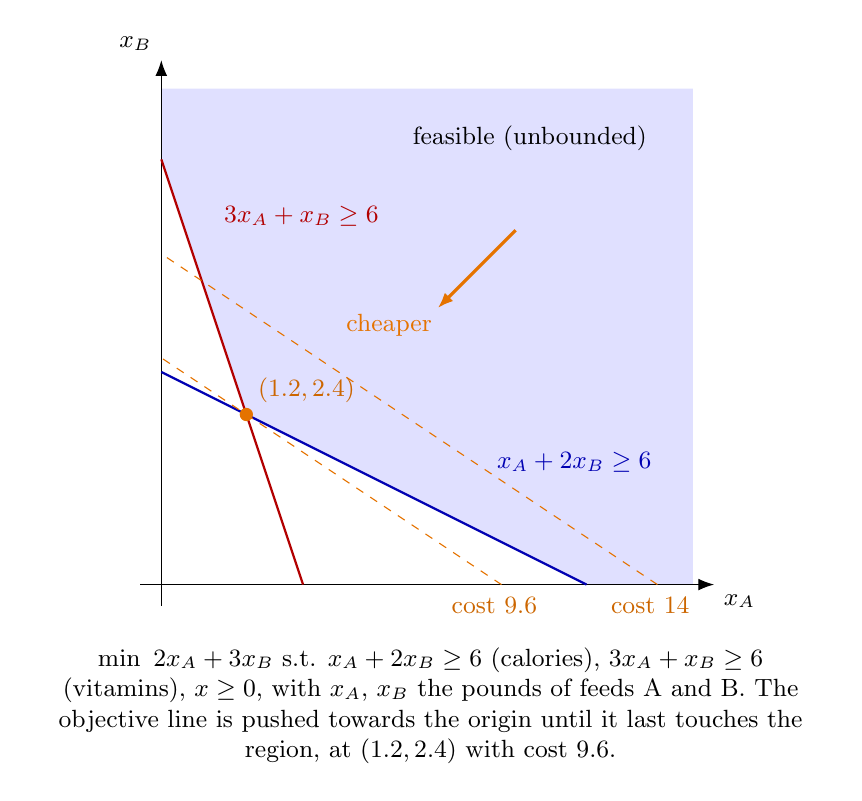
\begin{tikzpicture}[x=0.9cm, y=0.9cm, every node/.style={font=\small}, >={Latex[length=2mm]}]
	\fill[blue!12] (6,0) -- (7.5,0) -- (7.5,7) -- (0,7) -- (0,6) -- (1.2,2.4) -- cycle;
	\draw[->] (-0.3,0) -- (7.8,0) node[below right] {$x_A$};
	\draw[->] (0,-0.3) -- (0,7.4) node[above left] {$x_B$};
	\draw[blue!70!black, thick] (6,0) -- (0,3);
	\draw[red!70!black, thick] (2,0) -- (0,6);
	\node[blue!70!black, anchor=south west] at (4.6,1.45) {$x_A+2x_B\ge6$};
	\node[red!70!black, anchor=west] at (0.75,5.2) {$3x_A+x_B\ge6$};
	\draw[orange!90!black, dashed] (4.8,0) -- (0,3.2);
	\node[orange!80!black, anchor=north] at (4.7,-0.05) {cost $9.6$};
	\draw[orange!90!black, dashed] (7,0) -- (0,4.667);
	\node[orange!80!black, anchor=north] at (6.9,-0.05) {cost $14$};
	\draw[->, orange!90!black, very thick] (5.0,5.0) -- (3.9,3.9) node[below left, inner sep=1.5pt] {cheaper};
	\fill[orange!90!black] (1.2,2.4) circle (2.4pt);
	\node[orange!80!black, anchor=south west, inner sep=1.5pt] at (1.3,2.5) {$(1.2,2.4)$};
	\node at (5.2,6.3) {feasible (unbounded)};
	\node[anchor=north, align=flush center, text width=10cm] at (3.8,-0.75) {$\min\ 2x_A+3x_B$ s.t. $x_A+2x_B\ge6$ (calories), $3x_A+x_B\ge6$ (vitamins), $x\ge0$, with $x_A$, $x_B$ the pounds of feeds A and B. The objective line is pushed towards the origin until it last touches the region, at $(1.2,2.4)$ with cost $9.6$.};
\end{tikzpicture}
\end{document}
